\documentclass{article}
\usepackage{tabularx}
\usepackage{amsmath}
\usepackage{graphicx}
\usepackage[margin=2cm]{geometry}
\usepackage{cite}
\usepackage[final]{hyperref}
\usepackage{listings}
\usepackage{here}
\hypersetup{
	colorlinks=true,
	linkcolor=blue,
	citecolor=blue,
	filecolor=magenta,
	urlcolor=blue         
}

\begin{document}

\title{TP01\\Fractal}
\author{Robin Faury}
\date{12/15/20}
\maketitle

\begin{abstract}
	\begin{figure}[H]
		\centering
		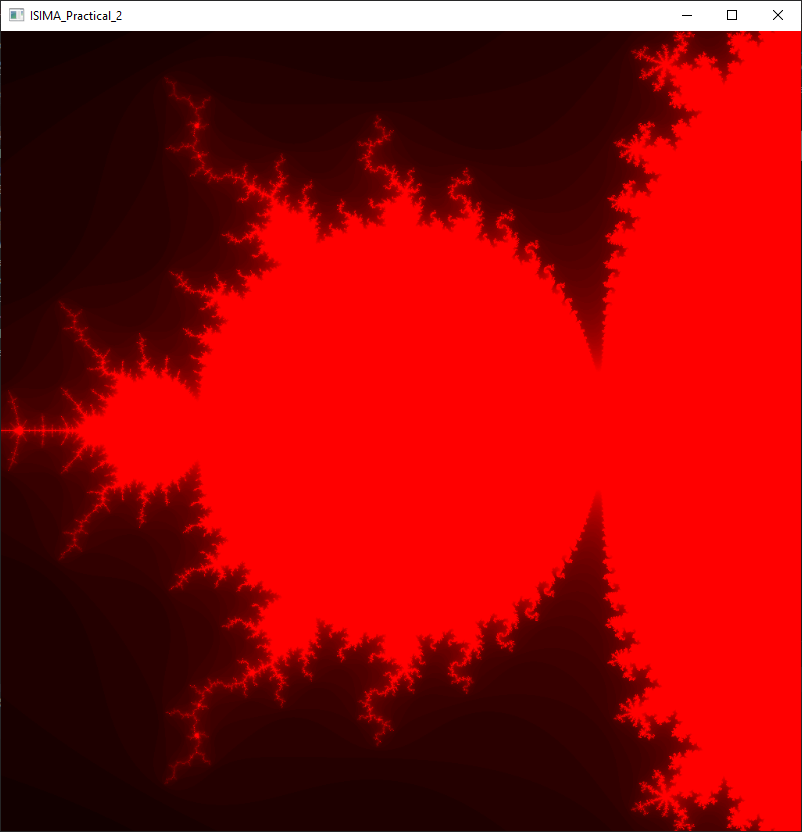
\includegraphics[scale=0.4]{images/Mandelbrot.png}
		\caption{The Mandelbrot set}
	\end{figure}
\end{abstract}

\newpage
\section{Introduction}
\subsection{Cloning the repository}
You can find the source of the practical work by cloning this git repository:
\begin{lstlisting}
	https://github.com/robinfaurypro/GPGPU_ISIMA_2020-2021.git
\end{lstlisting}
The CMakeLists file is stored into the Practical\_2 folder. Open a terminal on this folder and use thus commands:
\begin{lstlisting}
	git submodule update --init
	mkdir build
	cd build
	cmake -G "Visual Studio 15 Win64" ..
\end{lstlisting}
Of course if you are on UNIX system feel free to use the generator you want.
If everything is going well, you can compile and run the executable and get a gray window.


\end{document}